\documentclass[12pt]{article}
\textwidth=7in
\textheight=9.5in
\topmargin=-1in
\headheight=0in
\headsep=.5in
\hoffset=-.85in
\pagestyle{empty}
\usepackage{hyperref}
\renewcommand{\thefootnote}{\fnsymbol{footnote}}
\usepackage{graphicx}

\begin{document}
\begin{center}
{\bf Turn on the Red Light - A Simple Circuit}
\end{center}

\setlength{\unitlength}{1in}

\begin{picture}(6,.1) 
\put(-.25,0) {\line(1,0){7}}         
\end{picture}


\vskip.25in
\noindent\textbf{Objective:} Create a simple circuit using http://123d.circuits.io/. The circuit is to be powered with two $1.5v$ batteries in series with a resistor to provide a reasonable current per the LED specification provided below.

\vskip.25in
\noindent\textbf{LED Specification:} Use Red LEDs. Forward voltage is approximately $1.6$-$2.0V$. Forward current is approximately 10-20mA. Note that 1a is equivalent to 1000mA.

\vskip.25in
\noindent\textbf{Directions:} Select \textit{Create New Circuit} on the http://123d.circuits.io/circuits/ page. You will power your circuit with 3V. Select \textit{Components} to open a drawer at the bottom of the window, and then select and drag two \textit{AA batteries} to the prototyping area. You must connect this power source to the breadboard. To do so, connect the \textit{negative terminal} of one batter to the \textit{negative rail} (i.e., the line that is blue), and connect the \textit{positive terminal} of the other battery to the \textit{positive rail} (i.e., the line that is red). \\

\noindent{Question 1:} Currently you have the negative terminal of one battery connected to the negative rail, and the positive terminal of the other battery connected to the positive rail. Is this a complete circuit? \\

\noindent{You will want to connect the two batteries. To do so, connect the free positive terminal of one battery to the free negative terminal of the other. It should look similar to the following:} \\

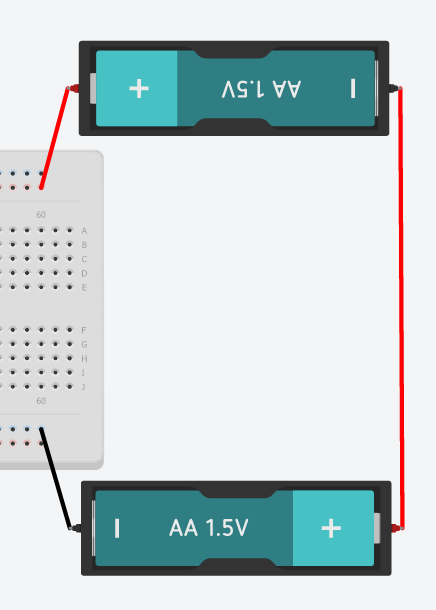
\includegraphics{battery.png} \\

\noindent{Question 2:} Why have we configured the battery in series and not in parallel? \\

\noindent{Next, select the LED component and drag it to an open space on the bread board (e.g., $A45$+$A45$). Note that the straight edge of the LED is the \textit{cathode} and the curved edge is \textit{anode}. Connect the cathode to the negative rail and connect the anode to the negative rail by clicking the respective location and dragging it. Click \textit{Start Simulation}. } \\

\noindent{Question 3:} You should have a complete circuit now! Congratulations. But, wait... does your LED look like it just exploded? Why did this happen? \\

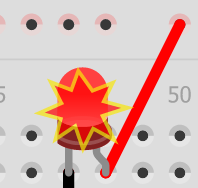
\includegraphics{explode_led.png} \\

\noindent{To solve our exploding LED we need to add another component --- a \textit{resistor}. Drag a resistor from the components drawer to the breadboard. Place the resistor such that one of its terminals is connected to the positive rail and the other is on A-E. Connect the LED anode to the resistor terminal on A-E. Click \textit{Start Simulation}.} \\

\noindent{Question 4:} The LED still explodes! The resistor defaults to 1 ohm. Recall that Current = Voltage / Resistance, or $I=V/R$. $I=3V/1\Omega$. Your current to the LED is $2A$ but should be $10$-$20mA$. What is a reasonable resistance value for our circuit? \\

\noindent{Drag an \textit{Arduino Uno} to your prototyping area. Add another Red LED to your breadboard (e.g., $A10$-$A11$}. Microcontroller boards like Arduino have external power sources and thus have pinouts for ground (GRND) and power ($3.3V$ and $5V$). Connect the anode of the LED to the 5.5V pin on the Arduino Uno, and connect the cathode to the GRND pin on the Arduino Uno. Click \textit{Start Simulation.} \\

\noindent{Question 4:} With an increased voltage, what is a reasonable resistance to avoid another LED explosion? You may use the image below to help you. Note that we blurred out the resistor color codes. \\
 
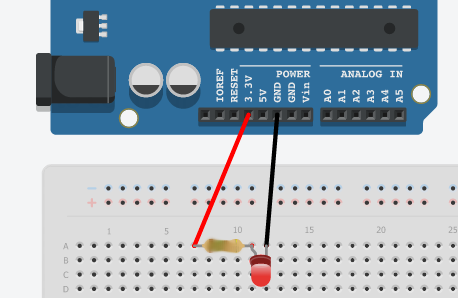
\includegraphics{arduino_led} \\
 
\end{document}
